\chapter{Psalm 44}

\begin{figure}
  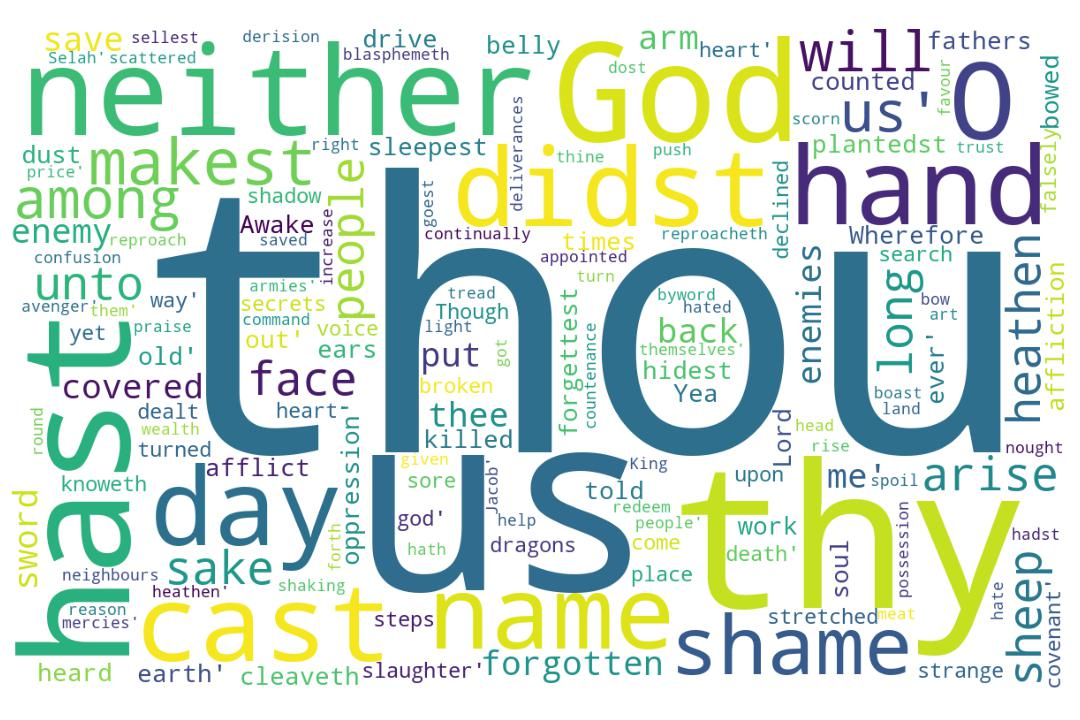
\includegraphics[width=\linewidth]{19OT-Psalms/Psalm44-WordCloud.jpg}
  \caption{Psalm 44 Word Cloud}
  \label{fig:Psalm 44 word Cloud}
\end{figure}

\marginpar{\scriptsize \centering \fcolorbox{bone}{lime}{\textbf{JACOB'S TROUBLES}}\\ (Psalm 44:1-26) \begin{compactenum}[I.][8]
    \item The \textbf{Son} of Perdition \index[scripture]{Psalms!Psa 044:01}(Psa 44:1)
    \item \textbf{Situation} Foretold %\index[scripture]{Exodus!Exodus 01:08}(Exodus 1:8)
    \item \textbf{Selah} Foretold \index[scripture]{Psalms!Psa 044:08}(Psa 44:8)
    \item Jews \textbf{Sacrificed} \index[scripture]{Psalms!Psa 044:11}\index[scripture]{Psalms!Psa 044:22}(Psa 44:11, 22)
    \item \textbf{Sold} into Slavery \index[scripture]{Psalms!Psa 044:12}(Psa 44:12)
    \item The \textbf{Shadow} of Death \index[scripture]{Psalms!Psa 044:23--24}(Psalm 44:23--24) (see also \index[scripture]{Exodus!Exo 01--03} Exodus 1--3, \index[scripture]{Job!Job 10:21--22}Job 10:21--22, \index[scripture]{Isaiah!Isa 09:02}Isa 9:2)
    \item The \textbf{Second} Advent Desired \index[scripture]{Psalms!Psa 044:26}(Psa 44:26)
\end{compactenum}}

\footnote{\textcolor[cmyk]{0.99998,1,0,0}{\hyperlink{TOC}{Return to end of Table of Contents.}}}\footnote{\href{https://audiobible.com/bible}{\textcolor[cmyk]{0.99998,1,0,0}{Psalms Audio}}}\textcolor[cmyk]{0.99998,1,0,0}{To the chief Musician for the sons of Korah, Maschil.}\\
\\
\textcolor[cmyk]{0.99998,1,0,0}{We have heard with our ears, O God, our fathers have told us, \emph{what} work thou didst in their days, in the times of old.}
[2] \textcolor[cmyk]{0.99998,1,0,0}{\emph{How} thou didst drive out the heathen with thy hand, and plantedst them; \emph{how} thou didst afflict the people, and cast them out.}%\marginpar{\scriptsize people, place, plantedst , possession, praise, price, push, put}
[3] \textcolor[cmyk]{0.99998,1,0,0}{For they got not the land in possession by their own sword, neither did their own arm save them: but thy right hand, and thine arm, and the light of thy countenance, because thou hadst a favour unto them.}\footnote{\textbf{Exodus 15:6} - Thy right hand, O LORD, is become glorious in power: thy right hand, O LORD, hath dashed in pieces the enemy.}\footnote{\textbf{Exodus 15:12} -  Thou stretchedst out thy right hand, the earth swallowed them.}%\marginpar{\scriptsize cast, cleaveth, come, command, confusion, continually, counted, countenance, covenant, covered}
[4] \textcolor[cmyk]{0.99998,1,0,0}{Thou art my King, O God: command deliverances for Jacob.}
[5] \textcolor[cmyk]{0.99998,1,0,0}{Through thee will we push down our enemies: through thy name will we tread them under that rise up against us.}
[6] \textcolor[cmyk]{0.99998,1,0,0}{For I will not trust in my bow, neither shall my sword save me.}
[7] \textcolor[cmyk]{0.99998,1,0,0}{But thou hast saved us from our enemies, and hast put them to shame that hated us.}
[8] \textcolor[cmyk]{0.99998,1,0,0}{In God we boast all the day long, and praise thy name for ever. \fcolorbox{bone}{lime}{Selah}.}\footnote{Compare with \textbf{Psalm 89:37-38} - It shall be established for ever as the moon, and as a faithful witness in heaven. Selah. [38] But thou hast cast off and abhorred, thou hast been wroth with thine anointed. Some things have to happen before the deliverances and triumphs spoken of in verses 4, 5, 7, and 8.} 
[9] \textcolor[cmyk]{0.99998,1,0,0}{But thou hast cast off, and put us to shame; and goest not forth with our armies.}
[10] \textcolor[cmyk]{0.99998,1,0,0}{Thou makest us to turn back from the enemy: and they which hate us spoil for themselves.}
[11] \textcolor[cmyk]{0.99998,1,0,0}{Thou hast given us like \fcolorbox{bone}{lime}{sheep \emph{appointed}} for meat; and hast \fcolorbox{bone}{lime}{scattered} us among the heathen.}\footnote{\textbf{Joel 3:2} -  I will also gather all nations, and will bring them down into the valley of Jehoshaphat, and will plead with them there for my people and for my heritage Israel, whom they have scattered among the nations, and parted my land.}
[12] \textcolor[cmyk]{0.99998,1,0,0}{Thou \fcolorbox{bone}{lime}{sellest} thy people for nought, and dost not increase \emph{thy} \emph{wealth} by their price.}\footnote{\textbf{Psalm 119:25} - My soul cleaveth unto the dust: quicken thou me according to thy word.}\footnote{\textbf{Lamentations 4:8} - Their visage is blacker than a coal; they are not known in the streets: their skin cleaveth to their bones; it is withered, it is become like a stick.}
[13] \textcolor[cmyk]{0.99998,1,0,0}{Thou makest us a reproach to our neighbours, a scorn and a derision to them that are round about us.}\footnote{\textbf{Job 30:1} - But now they that are younger than I have me in derision, whose fathers I would have disdained to have set with the dogs of my flock.}\footnote{\textbf{Psalm 79:4} -We are become a reproach to our neighbours, a scorn and derision to them that are round about us.}\footnote{\textbf{Psalm 119:51} - The proud have had me greatly in derision: yet have I not declined from thy law.}\footnote{\textbf{Ezekiel 36:4} - The proud have had me greatly in derision: yet have I not declined from thy law.}
[14] \textcolor[cmyk]{0.99998,1,0,0}{Thou makest us a byword among the heathen, a shaking of the head among the people.}\footnote{\textbf{Deuteronomy 28:38} - And now am I their song, yea, I am their byword.}\footnote{\textbf{Job 17:6} - He hath made me also a byword of the people; and aforetime I was as a tabret.}\footnote{\textbf{Job 30:9} - And now am I their song, yea, I am their byword.}
[15] \textcolor[cmyk]{0.99998,1,0,0}{My confusion \emph{is} continually before me, and the shame of my face hath covered me,}\footnote{\textbf{Ezra 9:7} - Since the days of our fathers have we been in a great trespass unto this day; and for our iniquities have we, our kings, and our priests, been delivered into the hand of the kings of the lands, to the sword, to captivity, and to a spoil, and to confusion of face, as it is this day.}\footnote{\textbf{Job 10:15} - If I be wicked, woe unto me; and if I be righteous, yet will I not lift up my head. I am full of confusion; therefore see thou mine affliction;}
[16] \textcolor[cmyk]{0.99998,1,0,0}{For the voice of him that reproacheth and blasphemeth; by reason of the enemy and avenger.}\footnote{\textbf{Psalm 8:2}  - Out of the mouth of babes and sucklings hast thou ordained strength because of thine enemies, that thou mightest still the enemy and the avenger.}
[17] \textcolor[cmyk]{0.99998,1,0,0}{All this is come upon us; yet have we not forgotten thee, neither have we dealt falsely in thy covenant.}
[18] \textcolor[cmyk]{0.99998,1,0,0}{Our heart is not turned back, neither have our steps declined from thy way;}
[19] \textcolor[cmyk]{0.99998,1,0,0}{Though thou hast sore broken us in the place of dragons, and covered us with the shadow of death.}\footnote{\textbf{Psalm 38:8} -  am feeble and sore broken: I have roared by reason of the disquietness of my heart.}
[20] \textcolor[cmyk]{0.99998,1,0,0}{If we have forgotten the name of our God, or stretched out our hands to a strange god;}
[21] \textcolor[cmyk]{0.99998,1,0,0}{Shall not God search this out? for he knoweth the secrets of the heart.}\footnote{\textbf{Jeremiah 17:10} -  I the LORD search the heart, I try the reins, even to give every man according to his ways, and according to the fruit of his doings.}\footnote{\textbf{1 Corinthians 14:25} - And thus are the secrets of his heart made manifest; and so falling down on his face he will worship God, and report that God is in you of a truth.}
[22] \textcolor[cmyk]{0.99998,1,0,0}{Yea, for thy sake are we killed all the day long; we are counted as sheep for the slaughter.}\footnote{\textbf{Jeremiah 12:3} - But thou, O LORD, knowest me: thou hast seen me, and tried mine heart toward thee: pull them out like sheep for the slaughter, and prepare them for the day of slaughter.}\footnote{\textbf{Romans 8:36} - As it is written, For thy sake we are killed all the day long; we are accounted as sheep for the slaughter.}
[23] \textcolor[cmyk]{0.99998,1,0,0}{Awake, why sleepest thou, O Lord? arise, cast \emph{us} not off for ever.}
[24] \textcolor[cmyk]{0.99998,1,0,0}{Wherefore hidest thou thy face, \emph{and} forgettest our affliction and our oppression?}\footnote{\textbf{Deuteronomy 26:7} - And when we cried unto the LORD God of our fathers, the LORD heard our voice, and looked on our affliction, and our labour, and our oppression:}\footnote{\textbf{Psalm 107:39} - Again, they are minished and brought low through oppression, affliction, and sorrow.}
[25] \textcolor[cmyk]{0.99998,1,0,0}{For our soul is bowed down to the dust: our belly cleaveth unto the earth.}\footnote{\textbf{Psalm 22:29} - All they that be fat upon earth shall eat and worship: all they that go down to the dust shall bow before him: and none can keep alive his own soul.}
[26] \textcolor[cmyk]{0.99998,1,0,0}{Arise for our help, and redeem us for thy mercies's sake.}\footnote{\textbf{Psalm 130:7-8} - Let Israel hope in the LORD: for with the LORD there is mercy, and with him is plenteous redemption. [8] And he shall redeem Israel from all his iniquities.}



